\documentclass[11pt]{beamer}
% => essayer différents thèmes (en décommantant une des trois lignes suivantes)
%\usetheme{PaloAlto}
\usetheme{Madrid}
%\usetheme{Copenhagen}
%\usetheme{Marburg}

% => il est possible, pour un thème donné, de modifier seulement la couleur
%\usecolortheme{crane}
\usecolortheme{seahorse}
\setbeamertemplate{background canvas}{
\includegraphics[width=\paperwidth,height=\paperheight]{page.jpg}}

\useoutertheme[left]{sidebar}

\usepackage[utf8]{inputenc}
\usepackage[T1]{fontenc}
\usepackage[english]{babel}
\usepackage{graphicx}
\newenvironment<>{examplefirst}[1]{%
  \setbeamercolor{block title}{fg=white,bg=red!75!black}%
  \begin{block}#2{#1}}{\end{block}}
\newenvironment<>{examplesecond}[1]{%
  \setbeamercolor{block title}{fg=white,bg=blue!75!black}%
  \begin{block}#2{#1}}{\end{block}}
  
\author{Mourad Daoudi}
\title{Les Réseaux de Pétri}
%\subtitle{}
%\logo{}
\institute{USTHB}
\date{Jeudi 25 Juin}
%\subject{}
%\setbeamercovered{transparent}
%\setbeamertemplate{navigation symbols}{}

\begin{document}
	\maketitle
	\begin{frame}[shrink=15]
		\frametitle{Sommaire}
		\tableofcontents{}
	\end{frame}
	\AtBeginSection[]{
		
		\begin{frame}[shrink=15]
				\frametitle{Sommaire}
				\tableofcontents[currentsection]
			\end{frame}
		
		}
		\AtBeginSubsection[]{
			
			\begin{frame}[shrink=15]
				\frametitle{Sommaire}
				\tableofcontents[currentsubsection]
			\end{frame}
			}
				\AtBeginSubsubsection[]{
						
						\begin{frame}[shrink=15]
							\frametitle{Sommaire}
							\tableofcontents[currentsubsection]
						\end{frame}
						}





	\section{Introduction}
		\begin{frame}
		\frametitle{Définition génerale}
	
	
		\begin{examplefirst} {Rappel d'histoire}
		Les réseaux de Petri ont été inventés par le mathématicien allemand Carl Alain Petri dans
			les années 1960.
		\end{examplefirst}
	
	
		
		
		\end{frame}
	
	\section{Notations et règles de franchissement}

	\subsection{ Places, Transitions et Arcs       }
		\begin{frame}
	\frametitle{Définitions}
	\begin{examplesecond} {Un réseau de pétri c'est quoi ?}
		\setbeamercovered{invisible}
	   \begin{itemize}
	   \item  \uncover<.1-> { un graphe}
	   \item \uncover<.2-> {formé de deux types de nœuds appelés places et transitions, reliés par des arcs orientés}
	   \item \uncover<.3->  {biparti, c.-à-d. qu’un arc relie alternativement une place à une transition et une transition à une place}
	   \end{itemize}
	   
	   
	\end{examplesecond}
	
	\setbeamercovered{transparent}
	\begin{examplefirst} {Remarques}
		\setbeamercovered{transparent}
			
			   \begin{itemize}
				   \item  \uncover<.4->{Une place \textbf{(pi )} modélise les ressources utilisées dans le système.}
				   \item \uncover<.5 ->{ Une transition \textbf{(ti )} modélise les actions sur les ressources.}
		
				   \end{itemize}
	\end{examplefirst}
		
	\end{frame}
	\begin{frame}
	\frametitle{Exemples}
	\begin{block}{Exemples}
	la place p1 est en entrée de la transition t1 et p2 est en sortie de t1 .
	\end{block}
	\centering
	\begin{center}
		\includegraphics<1>[scale=0.40]{petriPlaces.png}
	\end{center}
	
	
	\end{frame}
	\begin{frame}

	 	\begin{block}{Remarques}
	 	-Une transition sans place en entrée est une transition source.
	 	
	 	-Une transition sans place en sortie est une transition puits.
	 	\end{block}
	 	\centering
	 	\begin{center}
	 		\includegraphics<1>[scale=0.40]{PuitSource.png}
	 	\end{center}
	\end{frame}
	\subsection{ Marquages }
		\begin{frame} [shrink=15]
	\frametitle{Marquage}
	\begin{examplefirst} {Le Marquage}
	Chaque place \textbf{\textit{(pi )}} d’un RdP peut contenir un ou plusieurs marqueurs (jetons). 
	
	La configuration complète du réseau, avec toutes les marques positionnées, forme le marquage et définit
	l’état du réseau (et donc l’état du système modélisé).

	
	\end{examplefirst}
		\centering
		 	\begin{center}
		 		\includegraphics<1>[scale=0.40]{marquage.png}
		 	\end{center}
		 	\begin{itemize}
		 		\item P1 ,P2,P3 sont des places .
		 		\item T1 est une transition qui permet de passer de P1 vers Deux places P2 et P3 .
		 		\end{itemize}
	\end{frame}
	\subsection{ Franchissement             }
		\begin{frame}
	\frametitle{Franchissement}
	\textbf{Franchissement}
	
	C’est le formalisme qui permet de passer d’un marquage à un autre, ce qui rend compte de
	l’évolution du système modélisé. Une transition est franchissable si chacune des places en
	entrée compte au moins un jeton ; dans ce cas :
	\setbeamercovered{invisible}
	\begin{enumerate}
	\item \uncover<.1->{le franchissement est une opération indivisible (atomique)}
	\item \uncover<.2->{ un jeton est consommé dans chaque place en entrée}
	\item \uncover<.3->{ un jeton est produit dans chaque place en sortie}
	\end{enumerate}
	

	\end{frame}
		\begin{frame}{Exemples de franchissement}
	Voici des exemples de franchissement avec deux réseaux différents.

		
	
				\centering
					 	\begin{center}
					 		\includegraphics<1>[scale=0.32]{franchissement1.png}
					 	\end{center}
					 	
					 	\centering
					 		\begin{center}
					 				\includegraphics<1>[scale=0.32]{franchissement2.png}
					 		\end{center}
					 	
					 	
				
		\end{frame}
	\subsection{ Réseaux particuliers }
		\begin{frame}
		Il existe des réseaux particuliers on va dans la suite de ce cours  citer quelques uns .
	\frametitle{Graphe d'état}
	\begin{examplesecond}{Graphe d'état}
	 un graphe d'état a une particularité qui est relative à ses transitions tel que , chaque transition ne dispose que d’une place en entrée et une place en sortie.
	
	
	\end{examplesecond}
	
	\centering
						 	\begin{center}
						 		\includegraphics<1>[scale=0.32]{grapheetat.png}
						 	\end{center}
	
	
	\end{frame}
		\begin{frame}
		\frametitle{Réseau sans conflit}
			\begin{examplesecond}{Réseau sans conflit}
			   Un réseau sans conflit est un réseau où chaque place n’a qu’une transition en sortie.	
			\end{examplesecond}
				\centering
				\begin{center}
				\includegraphics<1>[scale=0.32]{sansconflit.png}
				\end{center}
    		
		\end{frame}
		
    	
    	\begin{frame}
		\frametitle{Réseau simple}
		\begin{examplesecond}{Réseau simple}
		Les réseaux dits simples sont des  réseaux avec conflit(s) où chaque transition n’intervient au	plus que dans une situation de conflit.
		\end{examplesecond}
				\centering
				\begin{center}
				\includegraphics<1>[scale=0.32]{simpleR.png}
				\end{center}
		\end{frame}
			

    	\begin{frame}
		\frametitle{Les Graphes purs}
		\begin{examplesecond}{Graphe pur}
		Les  Graphes purs sont ceux dont aucune place n'est à la fois en entrée ou en sortie de la même transition.
		\end{examplesecond}
				\centering
				\begin{center}
				\includegraphics<1>[scale=0.32]{graphepur.png}
				\end{center}
		\end{frame}
	\begin{frame}
		\frametitle{Notions et règles de franchissement }
		\begin{examplesecond}{Définition}
			 Un réseau de Petri est défini par le tuple \textbf{\textit{(P, T, Pré, Post, $M_{0}$ )}}
						
						\begin{itemize}
					\item 	\textbf{ P }: ensemble de places $p_{i}$
						\item  \textbf{ T }: ensemble de transitions
						\item \textbf{ Pré} : \textit{Pré(p, t)} est une valeur ($\geq$ 0) associée à l'arc allant de la place p à la transition t
						\item   \textbf{Post} : \textit{Post(p, t)} est une valeur ($\geq$ 0) associée à l'arc allant de la transition \textit{t} à la place \textit{p}
						\item  $M_{0}$ : vecteur décrivant le marquage initial, $M_{0}$  = ($M_{0}$  ($p_{1}$ ), . . . , $M_{0}$  ($p_{n}$)).
							 nombre de jetons dans la place $p_{1}$
							\end{itemize}
			\end{examplesecond}				
		\end{frame}
		\begin{frame}
				\frametitle{Notions et règles de franchissement }
	\textit{\textbf{Exemple}}
	     Soit P = $p_{1}$ , $p_{2}$ , $p_{3}$ où $p_{1}$ représente la ressource $«$fichier$»$, $p_{2}$ la ressource $«$imprimante$»$ et $p_{3}$ la ressource fichiers en cours d’impression.
	      On peut définir le RP suivant
		dans son état initial (par exemple).
			\begin{center}
						\includegraphics<1>[scale=0.5]{fichierimprimantes.png}
			\end{center}
		\end{frame}
\begin{frame}	{Exemple}	
		\textbf{	On a :}

		 Pré($p_{1}$ , t) = 1 (p donne le poids sur l’arc)
	
		Pré($p_{2}$  , t) = 1 ; 
		
		Pré($p_{3}$  , t) = 0
		
		P ost($p_{1}$  , t) = 0 ; 
		
		Post($p_{3}$ , t) = 0 ; 
		
		Post($p_{3}$ , t) = 1
		
		$M_{0}$  = ($M_{0}$ ($p_{1}$ ), $M_{0}$ ($p_{2}$), $M_{0}$  ($p_{3}$ )) = (5, 2, 0)

	\textbf{Remarque :}
	
	 dans le cas général, \textit{Pré(p, t)} représente le nombre de ressources de type p
		consommées par la transition \textit{t}, et \textit{Post(p, t) }représente le nombre de ressources de type \textit{p}
		produites suite au tir de la transition t.
		\textit{M (p)} indique le marquage de la place \textit{p} (nombre de jetons contenus dans \textit{p}).
		

		

\end{frame}
		
		

	
	\section{Propriétés des réseaux de Petri}
		\begin{frame} [shrink=10]
	\frametitle{Propriétés des réseaux de Petri}
	À partir du marquage initial, le réseau de Petri peut évoluer si les conditions sont vérifiées.
	
	\textbf{\textit{Exemple}} (se référer à l’exemple précédent) :
	
	 Soit $M_{0}$  = (5, 2, 0)
	Après le franchissement (tir) de la transition \textit{t}, on utilisera un fichier et une imprimante (car Pré($p_{1}$  , t) = 1 et Pré($p_{2}$  , t) = 1) et on aura un fichier en cours d’impression .

	\textbf{le marquage deviendra alors :}

	 $M_{1}$  = (4, 1, 1)
	 
	 Après un deuxième tir de la transition \textit{ t}, on obtiendra :
	 
	  $M_{2}$  = (3, 0, 2).
	
	 On ne peut plus effectuer
	un autre tir de t, car $M_{2}$  ($p_{2}$  ) = 0.
	
	Dans le cas général, pour un marquage \textit{M} , une transition \textit{t} est tirable si et seulement si pour tout \textit{p} $\in$ P , on a : $M_{p}$  $\geq$ Pré(p, t)
	La franchissabilité   (ou la sensibilisation ou le tir) d’une transition \textit{t} pour le marquage \textit{M} se	note : M [t>.
	
	Si le marquage résultant est $M^{'}$ , alors on note : $M_{}$ [t>$M^{'}$ .
	\end{frame}
	\begin{frame}{suite exemple }
	Dans l’exemple précédent :
	$M_{0}$ [t>$M_{1}$ ; $M_{1}$ [t>$M_{2}$ et \textit{t } n’est pas tirable pour $M_{2}$ car $M_{2}$ ($p_{2}$ ) < Pré($p_{2}$ , \textit{t}).

	Soit \textit{M} un marquage : M = (M ($p_{1}$ ), M ($p_{2}$ ). . . )
	
	\textbf{Notons:}
	
				$C^{-}$ la matrice des Prés telle que : $C^{-}$(ij) = Prés($p_{i}$  , $t_{j}$ )
	
	$C^{+}$ la matrice des P osts telle que: $C^{+}$ (ij) = Posts($p_{i}$  , $t_{j}$ )
	
\textbf{	 C = 	$C^{+}$ - $C^{-}$}
	
	Toujours dans l’exemple précédent on a: 
		\begin{center}
					
			\begin{minipage}[h]{0.4\linewidth}
	$C^{-}$ = Pré = 
				\(\begin{pmatrix}
							1 \\ 1 \\ 0
								\end{pmatrix}	\)				
			\end{minipage}
			\hspace{0.5cm}	
			\begin{minipage}[h]{0.4\linewidth}
		$C^{+}$ = Post = \(\begin{pmatrix}
										0 \\ 0 \\ 1
											\end{pmatrix}\)
							
			\end{minipage}
	
		\end{center}
	
	
				
	\end{frame}
	\begin{frame}{suite exemple(fichiers imprimantes)}
		\begin{center}
								\includegraphics<1>[scale=0.45]{fichierimprimantes.png}
			\end{center}
	Ainsi, avec cette notation, pour un marquage \textit{M} , une transition $t_{i}$  est tirable si et seulement
	si :
	
	 M $\geq$ ${}^iC^{-}$  , où ${}^iC^{-}$ est le vecteur colonne i de la matrice $C^{-}$ .
	
	
	
	\end{frame}
	\begin{frame}{suite exemple(fichiers imprimantes)}
	\begin{examplefirst}{Exemple (précédent suite)}

	$M_{1}$ est tirable car [4, 1, 1] $>$ [1, 1, 0] c.-à-d $M_{1}$ $>$ $t_{1}$ $C^{-}$
    $M_{2}$ n’est pas tirable car $M_{2}$  [3, 0, 2] n’est pas supérieur à 
$C^{-}$ [1, 1, 0]
	\begin{itemize}
	\item - Le tir d’une transition \textit{t} ou un marquage \textit{M} conduit à un nouveau marquage  	$M_{0}$  défini par :	$\forall$ p $\in$ P, $M_{0}$(\textit{p}) = \textit{M (p)} - \textit{Pré(p, t)} + \textit{Post(p, t)}
		où $M_{0}$ = M - ${}^tC^{-}$ + ${}^tC^{+}$ = M + ${}^tC$
	\end{itemize}
	
	
	\end{examplefirst}

\begin{examplesecond}{Application}
	$M_{1}$ = $M_{0}$ - ${}^tC^{-}$ + ${}^tC^{+}$
	
	$M_{1}$  = [5, 2, 0] - [1, 1, 0] + [0, 0, 1]
	
	$M_{1}$ = [4, 1, 1]
\end{examplesecond}

	\end{frame}
	\subsection{ Graphe de Marquage Accessible (GMA)}
		\begin{frame}
	\frametitle{Graphe de Marquage Accessible (GMA)}
	\begin{examplesecond}{Définition}
	
		Un marquage sera dit accessible si on peut l'atteindre à partir du marquage initial, soit directement (avec un seul tir), soit indirectement (avec plusieurs tirs).
		On note A l'ensemble des marquages accessibles d'un réseau de Petri.
	\end{examplesecond}
	
	\begin{center}
				
		
		\begin{minipage}[h]{0.5\linewidth}
		\textbf{	Exemple (précédent:fichiers \& imprimantes) : }\\
			A = $M_{0}$ , $M_{1}$  , $M_{2}$ \\
			Le graphe des marquages accessibles:
		\end{minipage}
		\hspace{0.5cm}
			\begin{minipage}[h]{0.3\linewidth}
					\includegraphics<1>[scale=0.6]{GMA_exemple.png}
				\end{minipage}

	\end{center}
	
	\end{frame}
	
	
	\begin{frame}
		\frametitle{Graphe de Marquage Accessible (GMA)}
		\textbf{Application}
		Considérons le réseau de Petri suivant :
		\begin{center}
			\includegraphics<1>[scale=0.51]{application1.png}
		\end{center}
	
		\end{frame}
		\begin{frame}{Application (suite)}
	
			
			soit T = ($t_{1},t_{2}$), on a:\\
			$C^{-}$ = Pré = 
		\(\begin{pmatrix}
					1 & 0 \\
					0 & 1 \\
					0 & 1 \\
					1 & 0
					\end{pmatrix}\)		
			$C^{+}$ = Post = 
			\(\begin{pmatrix}
									1 & 0 \\
									0 & 1 \\
									1 & 0 \\
									0 & 1
									\end{pmatrix}\)	
						
						
			C = $C^{+}$ - $C^{-}$ = 
			\(\begin{bmatrix}
									
									0 & 0 \\
									0 & 0 \\
									1 & -1 \\
									-1 & 1
									\end{bmatrix}\)	
${}^tC$ =	
    \(\begin{bmatrix}
        	0 & 0 & 1 & -1 \\ 0 & 0 & -1 & 1
    		\end{bmatrix}	
    \)				
						
						
		
		
		
	\end{frame}
	
	\begin{frame}
		\frametitle{Graphe de Marquage Accessible (GMA)}
		
		\textbf{Application}(suite)

		
	\begin{minipage}[h]{0.2\linewidth}
		\includegraphics<1>[scale=0.4]{application2.png}
	\end{minipage}
	\hspace{1cm}
	\begin{minipage}[h]{0.6\linewidth}
		avec M0 = (1, 1, 0, 4)\\
		On peut avoir les autres marquages accessibles,
		 exemple :
		$M_{0}$ [t1 >$M_{1}$ car [1, 1, 0, 4] > [0, 0, 1, -1]\\
		
		
		
		Donc :$M_{1}$  = $M_{0}$ + $^{t}C$ = [1, 1, 0, 4] + [0,0 ,1 ,-1] =[1,1,1,3] etc.\\
		Le graphe des marquages accessibles :
	\end{minipage}
	\end{frame}
	
	
	
	\subsection{ Le vecteur d’occurrence et l’équation de changement d’état }
		\begin{frame}
	\frametitle{Le vecteur d’occurrence et l’équation de changement d’état}
	\begin{examplesecond}

		Soit $T^{\ast}$ l’ensemble de transitions $T^{\ast}$ = $t_{1}$ , $t_{2}$ , . . . , $t_{n}$
		
		Soit S une séquence de transitions (S $\in$ $T^{\ast}$ ) ; $\overrightarrow{\sigma} = (\overrightarrow{\sigma} (t))_{t}$
		
		où $\overrightarrow{\sigma}$(t) est le nombre d’occurrences de t dans S.	
	\end{examplesecond}
	
	\textbf{Exemple 1 :}\\
	 Soit le graphe de marquage ci-dessous,\\
	
	\begin{minipage}[h]{0.2\linewidth}
	 	\includegraphics<1>[scale=0.4]{exemple_page9.png}
	\end{minipage}
	\hspace{1.5cm}
	\begin{minipage}[h]{0.6\linewidth}
		avec T = $t_{1}$ , $t_{2}$ , $t_{3}$.\\
			Considérons la séquence $\overrightarrow{\sigma}$ = $t_{1}$ $t_{2}$ $t_{3}$
			Alors le vecteur d'occurrences $\overrightarrow{\sigma} = (\overrightarrow{\sigma}$ ($t_{1}$ ), $\overrightarrow{\sigma}$ ($t_{2}$ ), $\overrightarrow{\sigma}$ ($t_{3}$ )) est $\overrightarrow{\sigma}$répétitives : $T_{ 1}$ $T_{ 2}$ $T_{ 3}$ $T_{ 4}$ et $T_{ 1}$ $T_{ 3}$ $T_{ 2}$ $T_{4}$
		
		= (2, 1, 0)
	\end{minipage}

	

 	\end{frame}
	
	\begin{frame}
		\frametitle{Le vecteur d’occurrence et l’équation de changement d’état}
		
			Ainsi, à partir d'un marquage M , on peut tirer une séquence de transitions $\sigma$, et on trouve
			le marquage $M^{'}$ .\\
			
		\begin{examplesecond}
			
			\centering
			L'équation de changement d'état est alors donnée comme suit :\\
			
			\textbf{$M_{0} = M + C . \overrightarrow{\sigma}$}
		\end{examplesecond}
		
	\end{frame}
	
	\begin{frame}
		\frametitle{Le vecteur d’occurrence et l’équation de changement d’état}
		
		\textbf{Exemple 2 :}
		le franchissement d'une transition «source» consiste à rajouter un jeton à chacune
		des places en sortie.\\
		
		\begin{center}
			\includegraphics<1>[scale=0.4]{exemple_page10_1.png}
		\end{center}
	\end{frame}
	
	\begin{frame}
		\frametitle{Le vecteur d’occurrence et l’équation de changement d’état}
		
		\textbf{Exemple 3 :}
		le franchissement d'une transition «puits» consiste à retirer un jeton de chacune
		de ses places en entrée.\\
		
		\begin{center}
			\includegraphics<1>[scale=0.4]{exemple_page10_2.png}
		\end{center}
	\end{frame}
	
	
		\begin{frame}
			\frametitle{Le vecteur d’occurrence et l’équation de changement d’état}
			
			\textbf{Exemple 4 :}\\
				séquence de franchissement :\\
				$M_{0}$ [t1 >$M_{1}$ avec $M_{1}$ = (0, 1, 0, 0)\\
				$M_{0}$ [t1 t2 >$M_{2}$ avec $M_{2}$ = (0, 0, 0, 1)\\
				$M_{0}$ [t1 t3 >$M_{3}$ avec $M_{3}$ = (0, 0, 0, 1)\\
				Ensemble des marquages accessibles : M $\ast$ = M0 , M1 , M1 , M3\\
			
			\begin{center}
				\includegraphics<1>[scale=0.35]{exemple_page10_3.png}
			\end{center}
		\end{frame}

	
	\subsection{ Quelques propriétés qualitatives                 }

	\subsubsection{ Bornitude                         }
		\begin{frame}
	\frametitle{Quelques propriétés qualitatives:Bornitude}


	

	\begin{examplesecond}{Définition:Bornitude}
		Une place sera dite k-bornée si $\forall M, M (p) \leq k$
	\end{examplesecond}
	
	\textbf{Exemple (précédent):}
	\begin{itemize}
	\item $M_{0}$(p1) = $M_{1}$(p1) = $M_{2}$(p1) = $M_{3}$(p1) = $M_{4}$(p1) = 1 donc p1 est 1-bornée\\
	\item la place p4 est 4-bornée
    \end{itemize}
		\begin{center}
				\includegraphics<1>[scale=0.29]{application1.png}
			\end{center}    
	

	
	\end{frame}
	
	\begin{frame} {Bornitude(suite)}
	\begin{examplesecond}
     
     Un réseau de Petri est borné s'il existe une valeur k telle que :
		\centering
		$\forall M,\forall p, M (p) \leq k$
	\end{examplesecond}
		\begin{examplefirst}{Remarque}
			Pour que le réseau soit borné, il faut que son ensemble de marquages accessibles
			A soit fini (sinon, le réseau n'est pas borné).
		\end{examplefirst}
		
		\textbf{Exemple :}
		\begin{center}
			\includegraphics<1>[scale=0.35]{exemple_page11.png}\\
			Réseaux non borné \hspace{2cm} Réseau 2-borné
		\end{center}
	\end{frame}
	\subsubsection{ Pseudo-vivacité                      }
	\begin{frame}
		\frametitle{Quelques propriétés qualitatives:Pseudo-vivacité}

		
		\textbf{Pseudo-vivacité   }
		\begin{examplesecond}{Définition}
			Le réseau de Petri est pseudo-vivant si $\forall M, \exists t / M [t >$
			c.-à-d. pour tout marquage, il existe au moins une transition tirable à partir de ce marquage.\\
			Ainsi, le GMA d'un RdP pseudo-vivant possède au moins un arc (transition) sortant de chaque
			état (marquage).
		\end{examplesecond}
		\begin{examplefirst}{Remarque}
			Un réseau pseudo vivant n'a pas de marquage puits (ou mort) c.-à-d. un marquage sans
			transition tirable. Donc s'il y a un marquage à partir duquel on ne peut pas tirer une transition
			alors le réseau n'est pas pseudo-vivant.
		\end{examplefirst}
	\end{frame}
	\subsubsection{ Quasi-vivacité    }
	\begin{frame}
		\frametitle{Quelques propriétés qualitatives:Quasi-vivacité }
	%	\textbf{Quasi-vivacité}
		\begin{examplesecond}{Définition :Quasi-vivacité}
			Un réseau est quasi-vivant si : $\forall$ t, $\exists$ M/M [t >
			c-à-d que pour toute transition, il existe au moins un marquage à partir duquel on peut
			tirer cette transition.
			
			 Ainsi, la quasi-vivacité désigne la possibilité de franchir au moins une
			fois chaque transition.
		\end{examplesecond}
	\end{frame}
	\subsubsection{ Vivacté                          }
		\begin{frame}
	\frametitle{Quelques propriétés qualitatives:Vivacité }
	
	
	\textbf{Vivacité}
	\begin{examplesecond}{Définition}
		Un RdP est vivant s'il est pseudo-vivant et quasi-vivant.
	\end{examplesecond}
	
	\textbf{Exemple:}
	\begin{center}
		\includegraphics<1>[scale=0.35]{vivacite.png}\\
		Réseau vivant.
	\end{center}
	\end{frame}
	
	\subsubsection{ Réseau sans blocage }
		\begin{frame}
	\frametitle{Quelques propriétés qualitatives:Réseau sans blocage }
	
	
	\textbf{Réseau sans blocage}
	\begin{examplesecond}{Définition}
		Un RdP est dit sans blocage s'il n'a pas de marquage puits (mort).\\
	\end{examplesecond}
	
	\textbf{Exemple:}
	\begin{center}
		\includegraphics<1>[scale=0.35]{reseauSansBlocage.png}\\
	\end{center}
	\end{frame}
	\subsubsection{ Etat d’accueil }
	\begin{frame}
		\frametitle{Quelques propriétés qualitatives:Etat d’accueil }
		
		
		\textbf{Etat d’accueil }
		\begin{examplesecond}{Définition}
			Un RdP admet un état d’accueil $M_{a}$ si :$ \forall M \in A, \exists \sigma \in T \ast /M [ \sigma > M_{a}$.\\
			c.-à-d. un marquage d'accueil $M_{a}$ est tel qu'on peut lui accéder à partir de n'importe quel
			autre marquage M via une séquence de transition $\sigma$.\\
		\end{examplesecond}
		
		\begin{examplefirst}{Remarque 1:}
			Un état d'accueil est accessible quelque soit l'évolution du réseau.\\
		\end{examplefirst}
	\end{frame}
	
	\begin{frame}
		\begin{examplefirst}{Remarque 2:}
			Si le marquage initial ($M_{0}$) est un marquage d'accueil, alors le réseau est dit réinitialisable.\\
		\end{examplefirst}
		\frametitle{Quelques propriétés qualitatives:Etat d’accueil}
		\textbf{Exemple:}
		\begin{center}
			\includegraphics<1>[scale=0.35]{etatAccueil.png}\\
			Réseau réinitialisable
		\end{center}
	\end{frame}
	\subsubsection{ Conservation                       }
		\begin{frame}
	\frametitle{Conversation}
	\begin{examplesecond}{Définition:Réseau de Petri conservatif}
	Un réseau de Petri est conservatif si :
	\begin{center}
	$\forall M \in A ,\sum_{i=1}^{size(P)} M_{0}(p_{i}) = \sum_{i=1}^{size(P)} M(p_{i})$

	\end{center}


		\end{examplesecond}
	\textbf{Exemple :}
	
	 Considérons le RdP tel que :
	 
	$M_{0}$ = [5, 8, 3] ; 5+8+3=16
	
	$M_{1}$ = [4, 6, 6] ; 4+6+6=16
	
	$M_{2}$= [3, 7, 6] ;  3+7+6=16
	
	Ce réseau est dit conservatif.
	\end{frame}
	\subsection{ Types de réseaux de Petri                    }

	\subsubsection{ Réseaux de Petri généralisés               }
			\begin{frame}{Réseaux de Petri généralisés}
		 \begin{examplesecond}{Définition}
		 Dans ces réseaux, des poids sont associés aux arcs.
		 
		 \end{examplesecond}
		 
		 \textbf{Exemple:}
		 \begin{center}
		 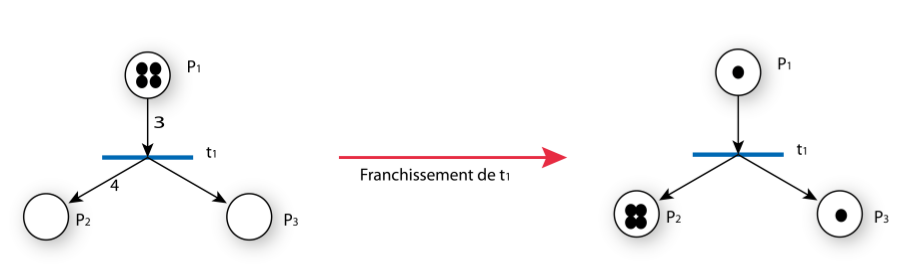
\includegraphics[scale=0.32]{petrigeneralisee.png}
		 \end{center}
		 
			\end{frame}
	\subsubsection{ Réseaux de Petri à capacités              }
		\begin{frame}{ Réseaux de Petri à capacités              }

		 \begin{examplesecond}{Définition}
			Dans ces réseaux, des poids sont associés aux places.
			 
			 \end{examplesecond}
			 
			 \textbf{Exemple:}
			 \begin{center}
			 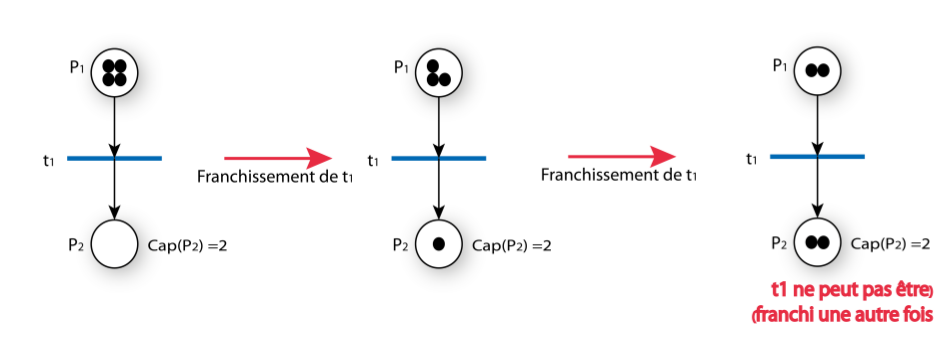
\includegraphics[scale=0.32]{petriacapacites.png}
			 \end{center}
	
	\end{frame}
	
		\subsubsection{ Réseaux de Petri à priorité                 }
			\begin{frame}{ Réseaux de Petri à priorité                 }
	
			 \begin{examplesecond}{Définition}
			Dans ces réseaux, on franchit la transition avec la plus grande priorité.
				 \end{examplesecond}
				 
				 \textbf{Exemple:}
				 \begin{center}
				 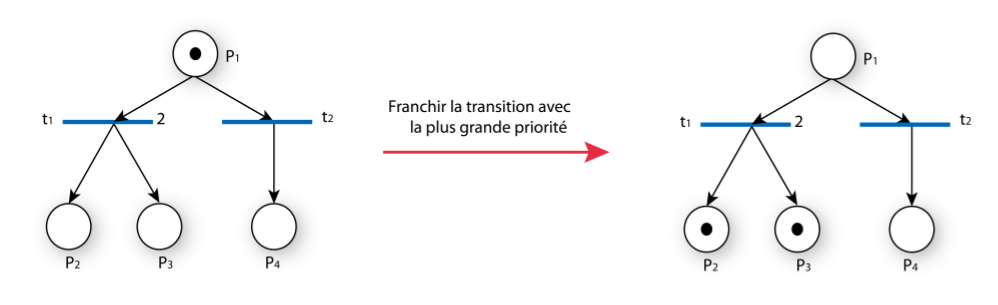
\includegraphics[scale=0.30]{petriapriorite.png}
				 \end{center}
		\end{frame}
	
	\subsubsection{ Graphe de marquage                   }
		\begin{frame}{ Graphe de marquage                   }

		 \begin{examplesecond}{Définition}
			À utiliser quand le nombre de marquages accessibles est fini.
		 \end{examplesecond}
			 
			 \textbf{Exemple: ici ya une erreur sur le graphe de marquage (non respect de la priorité à refaire)}
			 \begin{center}
			 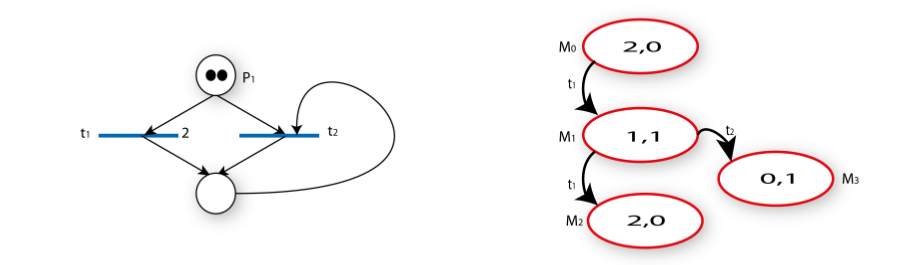
\includegraphics[scale=0.35]{graphemarquage.png}
			 \end{center}
	\end{frame}
	
	\begin{frame} {Graphe de marquage (propriétés)}
	Les propriétés déterminées à partir de ce graphe de marquages sont :
	\begin{itemize}
	\item 1 blocages : $M_{2}$ .
	\item  2-borné.
	\item  non-vivant (non peusdo-vivant : $\forall M, \exists t/M [t >)$
	\item  quasi-vivant ($ \forall t, \exists M/M [t > $)
	\item non réinitialisable (on ne peut pas trouve à partir d’un marquage une séquence de
		transition pour retrouver un marquage $M_{0}$ )
	\end{itemize}

	
	\end{frame}
	\subsection{ Arborescence de couverture                   }
		\begin{frame}{Arborescence de couverture}
		\begin{examplesecond}{Définition}
		Un graphe de marquage ne peut plus être construit quand le réseau est non borné c.-à-d.
		quand le nombre de marquages accessibles est infini.
		
		 D’où le recours au graphe de couverture.
		C’est un graphe à nombre de marquages fini.
		\end{examplesecond}
		

	\end{frame}
	\subsubsection{ Algorithme de construction d’un graphe de marquage}
		\begin{frame}[shrink=10]{Algorithme de construction d’un graphe de marquage}
\textbf{Pas 1 :} 

À partir du marquage initial $M_{0}$ , indiquer toutes les transitions validées et les mar-
quages accessibles successeurs correspondants.
Si un des marquages est strictement supérieur à $M_{0}$ , on met la variable "w" pour chacun des
composantes supérieures aux composantes de $M_{0}$ .

\textbf{Pas 2 :}

 Pour chaque nouveau marquage $M_{i}$ , on fait soit le pas 2.1, soit le pas 2.2
\begin{enumerate}
\item Pas 2.1 : S’il existe sur le chemin de $M_{0}$ jusqu’à $M_{i}$ (exclu) un marquage $M_{j}$ = $M_{i}$ ,
alors $M_{i}$ n’a pas de successeur.
\item Pas 2.2 : Sinon, on prolonge le graphe avec les successeurs $M_{k}$ ($M_{i}$ ) : une com-
posante "w" de $M_{i}$ reste une composante de "w" de $M_{k}$ .
S’il existe un marquage $M_{j}$ sur le chemin de $M_{0}$ à $M_{k}$ tel que $M_{k} > $  $M_{j}$ , alors on
met "w" pour chacune des composantes supérieure aux composantes de $M_{i}$ .
 
\end{enumerate}


	\end{frame}
	\begin{frame}{Algorithme de construction d’un graphe de marquage}
	\begin{examplesecond}
	
	\textbf{Opérations sur "w" (nombre très grand):}
	
	\begin{center}
	$  _\forall n \in \mathbb{N} , n < \infty   $
		\end{center}
	\textbf{Équation fondamentale:}
	\begin{center}
	$\left\lbrace\begin{array}{lll}
	n + w + w + n = w + w&=& w\\
	w - n&=& n
	\end{array}\right.$
	\end{center}

	
	\end{examplesecond}
	
	\end{frame}
	\begin{frame}{Exemple(Algorithme de construction  d'un graphe de marquage)}
\textbf{	Exemple :}
\begin{center}

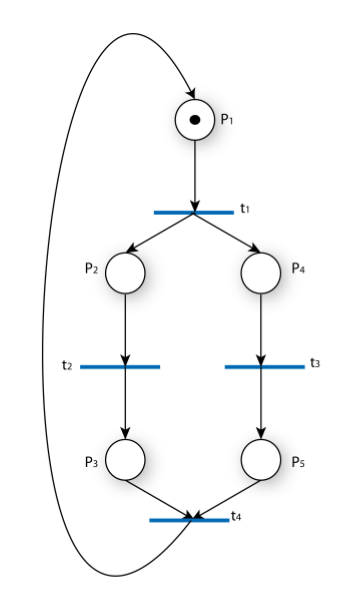
\includegraphics[scale=0.33]{algoPetri.png}
\end{center}

	\end{frame}

	\begin{frame} {Exemple(suite)}
		Soit la séquence $\sigma$ = $t_{1}$ $t_{2}$ , donc $\overrightarrow{\sigma}$ = (1, 1, 0, 0, 0)
	
		$C^{-}$ = 
		\( \begin{pmatrix}
	1&0&0&0\\0&1&0&0\\0&0&1&1\\0&0&0&1\\0&0&0&1
	\end{pmatrix}\)
		$C^{+}$ = 
	\( \begin{pmatrix}
	0&0&0&1\\1&0&0&0\\1&0&0&0\\0&1&0&0\\0&0&1&0
	\end{pmatrix}\)
	
		C = $C^{+}$- $C^{-}$ =  
	\( \begin{pmatrix}
	-1&0&0&1\\1&-1&0&0\\1&0&-1&0\\0&1&0&-1\\0&0&1&-1
	\end{pmatrix}\)
	
	L’équation fondamentale correspondant à cette séquence est :
	\begin{center}
	
	$M_{2}$ = $M_{0}$ + C · $\overrightarrow{\sigma}$
	
	\end{center}
	
	\end{frame}
	\begin{frame}
	 $M_{2}$ = \( \begin{pmatrix}
	 1\\0\\0\\0\\0\\
	 \end{pmatrix}\) + \( \begin{pmatrix}
	 	-1&0&0&1\\1&-1&0&0\\1&0&-1&0\\0&1&0&-1\\0&0&1&-1
	 	\end{pmatrix}\).\( \begin{pmatrix}
	 	1\\1\\0\\0\\0\\
	 	\end{pmatrix}\)
	 	= \( \begin{pmatrix}
	 	1\\0\\0\\0\\0\\
	 	\end{pmatrix}\) +
	 	\( \begin{pmatrix}
	 	-1\\0\\1\\1\\0\\
	 	\end{pmatrix}\)
	 	 $M_{2}$ = \( \begin{pmatrix}
	 	0\\0\\1\\1\\0\\
	 	\end{pmatrix}\)
	\end{frame}
	\begin{frame} {Exemple (suite :GMA)}
	\textbf{Graphe de marquage}
	
		\begin{minipage}[h]{0.3\linewidth}
			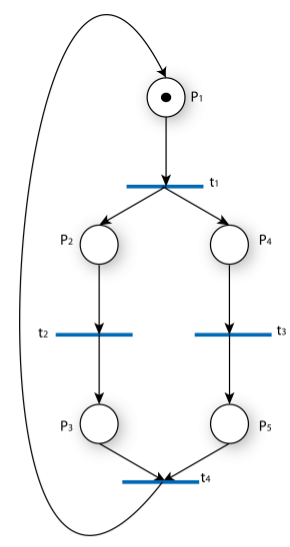
\includegraphics[scale=0.35]{treeexample.png}
			\end{minipage}
		\hspace{2cm}
		\begin{minipage}[h]{0.4\linewidth}
		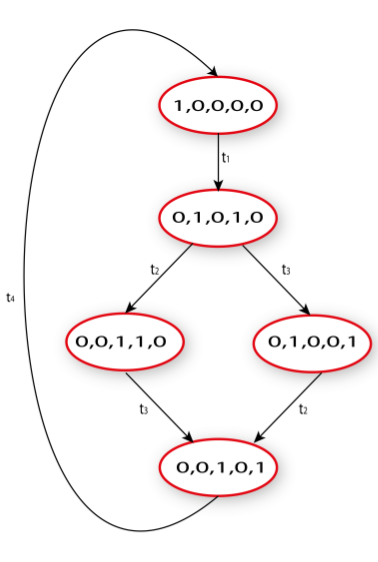
\includegraphics[scale=0.35]{treeexamplegma.png}
		\end{minipage}
		\end{frame}

    \begin{frame}{Exemple(suite:GMA)}
	\begin{examplesecond} 
	
	Propriétés 
	\begin{enumerate}
	\item sauf
	\item sans blocage
	\item réinitialisable : $M_{0}$ est un état d’accueil
	\item  2 séquences répétitives : $T_{1}$ $T_{2}$ $T_{3}$ $T_{4}$ et $T_{1}$ $T_{3}$ $T_{2}$ $T_{4}$
	\end{enumerate}

	\end{examplesecond}    
    \end{frame}

	

	
\end{document}